% Be sure to write chapter titles in ALL CAPS
\chapter{\uppercase{BACKGROUND}}

This chapter is divided into five main sections. First, I provide background on the Tor anonymity network and describe how clients can contact hidden services inside it. Secondly, I explain Bitcoin and its architecture as a prerequisite for Namecoin. Third, I detail Namecoin and compare and contrast with Bitcoin. Fourth, I provide an overview of traditional DNS and how it is used on the clearnet, and finally I introduce Zooko's Triangle: a conjecture that makes claims on the limits of persistent name systems.



\section{Tor}

The Tor network is a second-generation onion routing system that aims to provide anonymity, privacy, and Internet censorship protection to its users. Tor routes encrypted TCP/IP user traffic through a worldwide volunteer-run network of over six thousand relays. Tor's encryption, authentication, and routing protocols are designed to make it very difficult for any adversary to identify an end user or correlate them to their traffic. Tor continues to be one of the most popular and secure tools to use against network surveillance, traffic analysis, and information censorship.

\subsection{Design}

Tor provides an anonymity and privacy layer by relaying all end-user TCP traffic through a series of relays on the Tor network. Typically this route consists of a carefully-constructed three-hop path known as a \textit{circuit}, which changes over time. These nodes in the circuit are commonly referred to as \textit{guard node}, \textit{middle relay}, and the \textit{exit node}, respectively. Only the first node is exposed to the origin of TCP traffic into Tor, and only the exit node can see the destination of traffic out of Tor. The middle router, which passes encrypted traffic between the two, is unable to determine either. As such, each node is only aware of the machines it talks to, and only the client knows the identity of all three nodes used in its circuit. Tor's architecture thus minimizes the security risk from compromised nodes.\cite{McCoy2008}

Tor also contains nine authority nodes that maintain a list of IPs, ports, public keys, status, capability flags (entry guard, exit, etc) and other information on all Tor nodes in the network. This list is then signed by these nodes and periodically copied across all Tor nodes so that all Tor nodes can contact and authenticate to all other Tor nodes in the network.

\subsection{Routing}

In traditional Internet connections, the client communicates directly with the server. In this model, an eavesdropper can often reveal both the identity of the end user and their activities. Direct encrypted connections do not hide IP headers, which expose source and destination addresses and the size of the payload. In the face of adversaries with sophisticated traffic analysis tools, such information can be very revealing for someone who wishes to hide their online activities.

Tor combats this by routing end user traffic through a randomized circuit through the network of relays. The Tor client software first queries a trusted directory server or a relay mirroring the directory. This directory contains of list of IPs, ports, public keys, and other information about all nodes in the Tor network.\cite{Xin2009} Next, the Tor client chooses three unique and geographically diverse nodes to use. It then builds and extends the circuit one node at at time, negotiating respective HTTPS connections with each node in turn. No single relay knows the complete path, and each relay can only decrypt its layer of decryption. In this way, data is encrypted multiple times and then is decrypted in an onion-like fashion as it passes through the circuit.

\begin{figure}[htdp]
	\begin{minipage}[b]{0.45\linewidth}
		\centering
		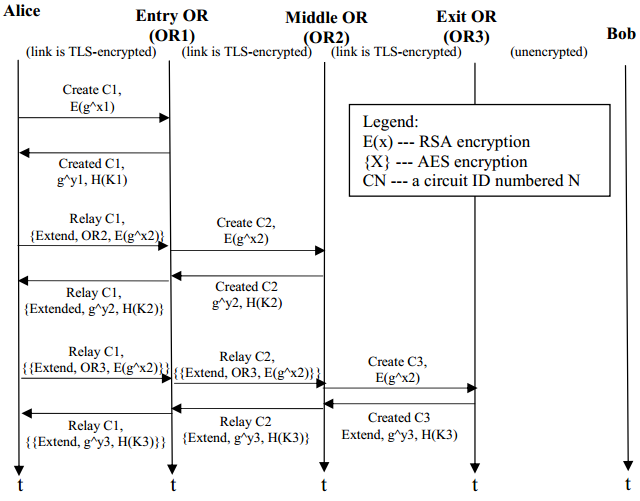
\includegraphics[width=\textwidth]{images/circuit-construction.png}
		\caption{Anatomy of the construction of a Tor circuit.}
		\label{fig:figure1}
	\end{minipage}
	\hspace{0.5cm}
	\begin{minipage}[b]{0.45\linewidth}
		\centering
		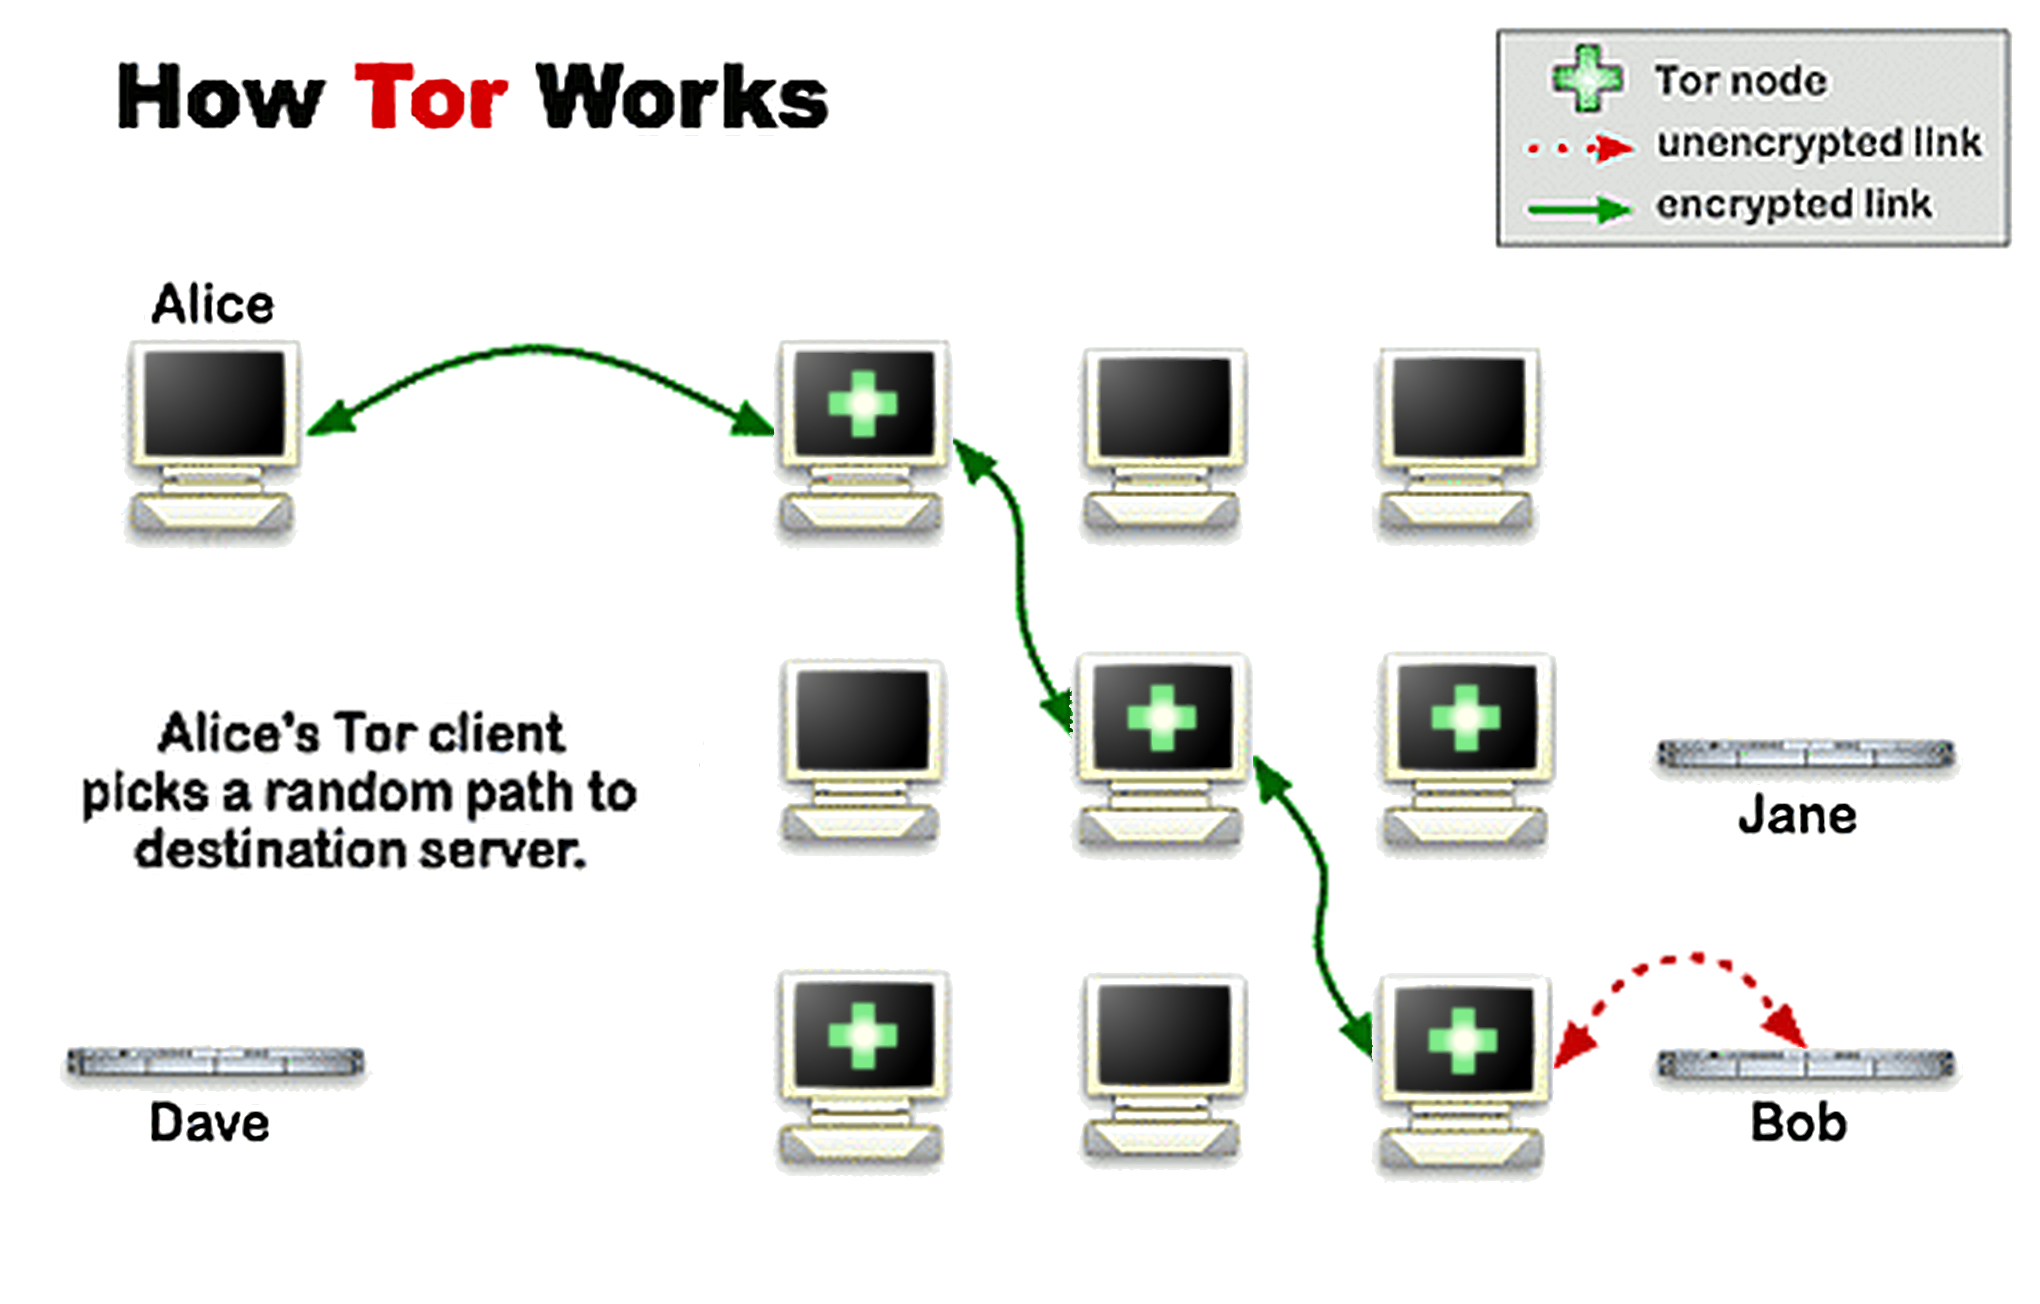
\includegraphics[width=\textwidth]{images/circuit-building-2-5.png}
		\caption{A circuit through the Tor network.}
		\label{fig:figure2}
	\end{minipage}
\end{figure}

The client first establishes a TLS connection with the first relay, $R_{1}$, using the relay's public key. The client then performs a Diffie-Hellman-Merkle key exchange to negotiate $K_{1}$ which is then used to generate two symmetric session keys: a forward key $K_{1,F}$ and a backwards key $K_{1,B}$. $K_{1,F}$ is used to encrypt all communication from the client to $R_{1}$ and $K_{1,B}$ is used for all replies from $R_{1}$ to the client. These keys are used conjunction with the symmetric cipher suite negotiated during the TLS handshake, thus forming an encrypted tunnel with perfect forward secrecy. Once this one-hop circuit has been created, the client then sends $R_{1}$ the RELAY\_EXTEND command, the address of $R_{2}$, and the client's half of the Diffie-Hellman-Merkle protocol using $K_{1,F}$. $R_{1}$ performs a TLS handshake with R${2}$ and uses $R_{2}$'s public key to send this half of the handshake to $R_{2}$, who replies with his second half of the handshake and a hash of $K_{2}$. $R_{1}$ then forwards this to the client under $R_{1,B}$ with the RELAY\_EXTENDED command to notify the client. The client generates $K_{1,F}$ and $K_{1,B}$ from $K_{2}$, and repeats the process for $R_{3}$,\cite{Ling2012} as shown in Figure 3. The TLS/IP connections remain open, so the returned information travels back up the circuit to the end user.

Following the complete establishment of a circuit, the Tor client software then offers a Secure Sockets (SOCKS) interface on localhost which multiplexes TCP traffic through Tor. At the application layer, this data is packed and padded into equally-sized Tor \textit{cells}, transmission units of 512 bytes. As each relay sees no more than one hop in the circuit, in theory neither an eavesdropper nor a compromised relay can link the connection's source, destination, and content. Tor further obfuscates user traffic by changing the circuit path every ten minutes,\cite{McCoy2008} as shown in Figure 4. A new circuit can also be requested manually by the user.

\begin{figure}[htbp]
	\centering
	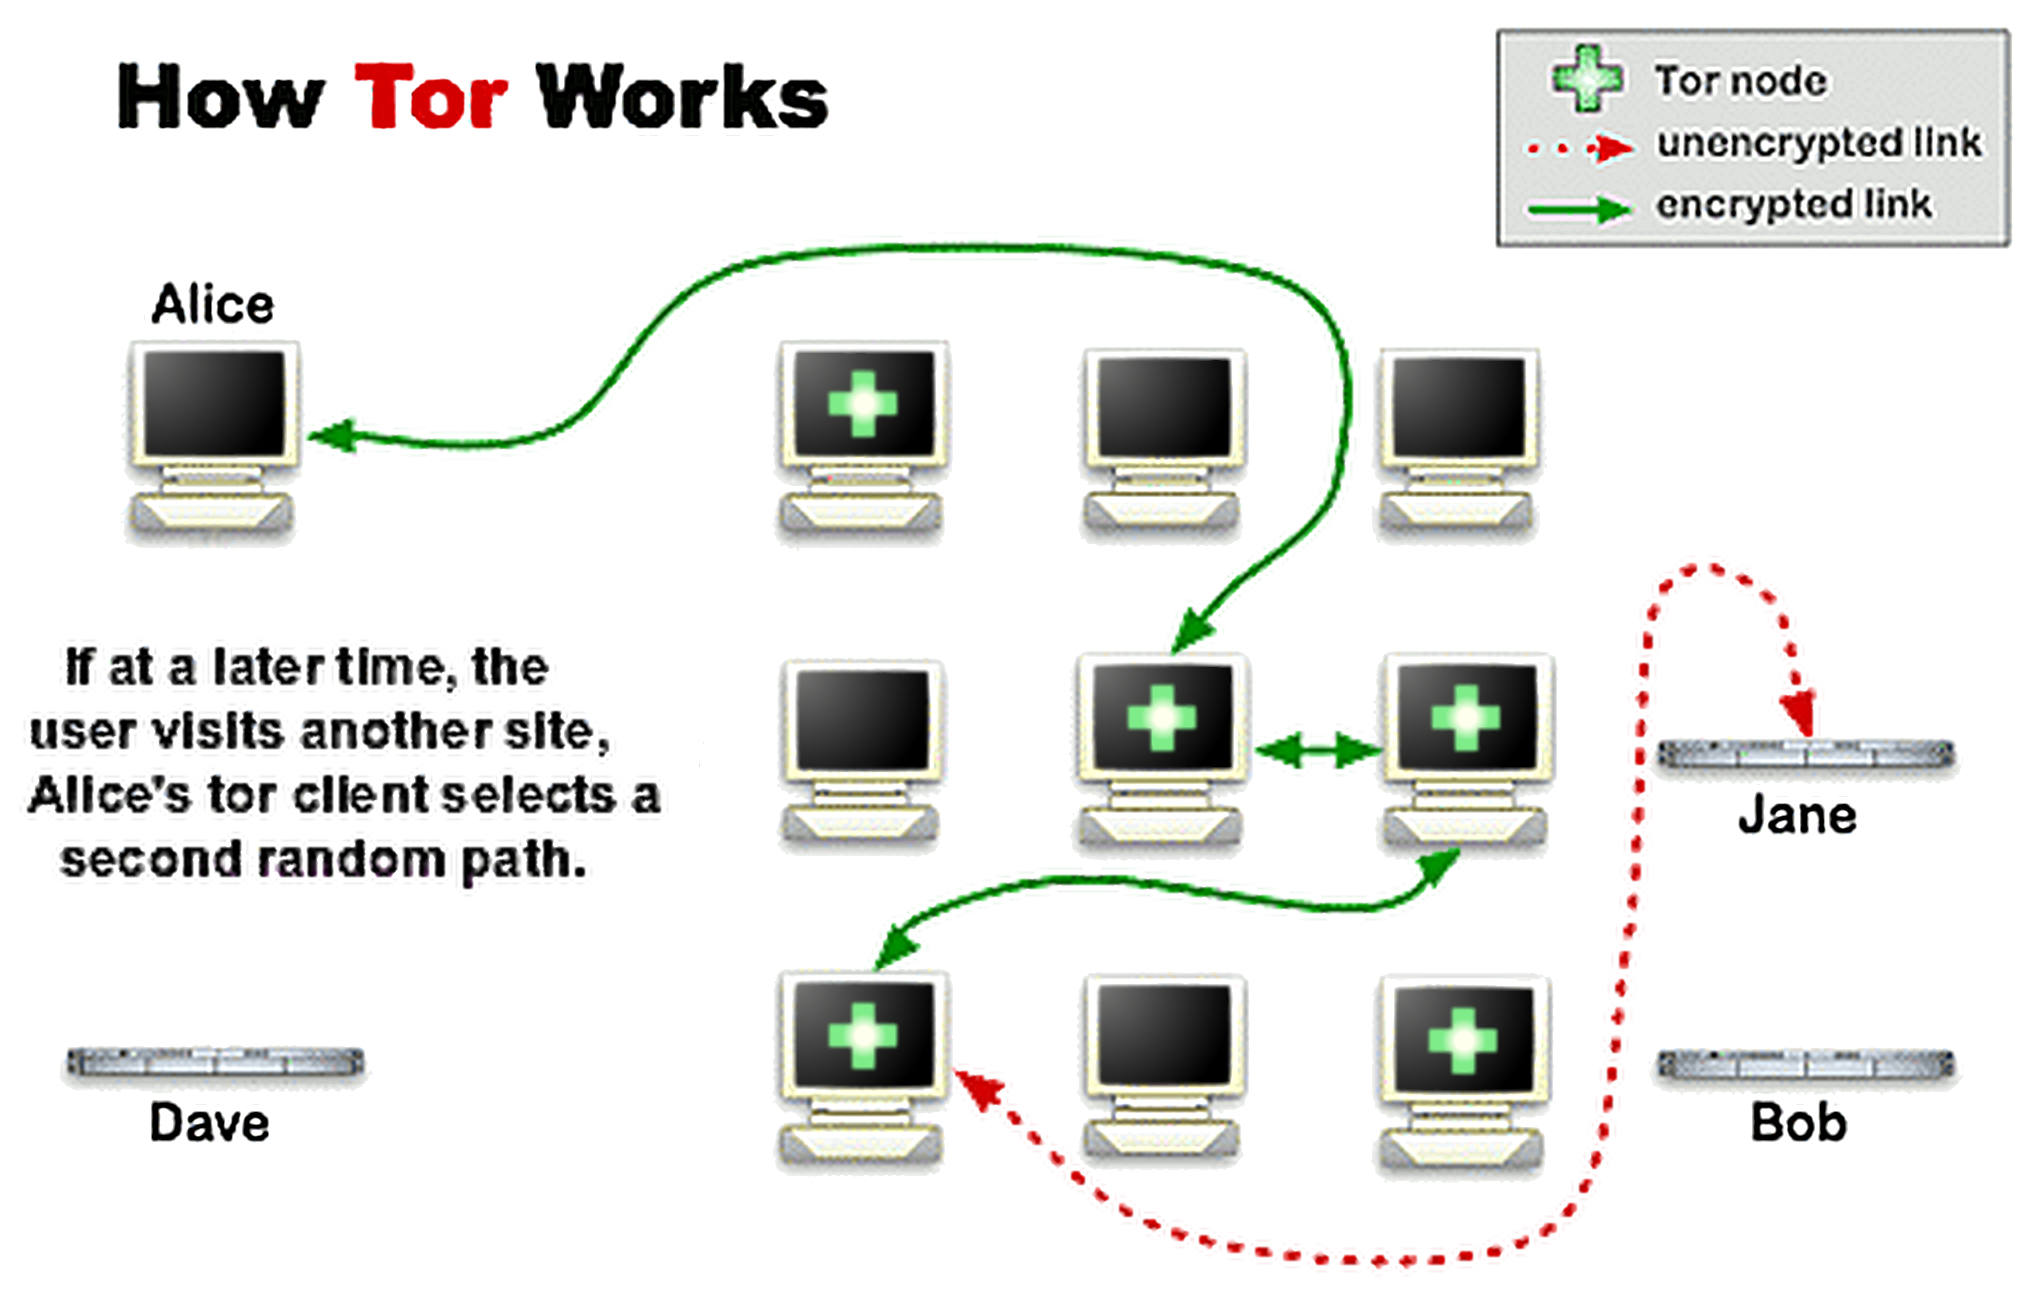
\includegraphics[width=0.6\textwidth]{images/circuit-change-1-4.png}
	\caption{A Tor circuit is changed periodically, creating a new user identity.}
	\label{fig:figure3}
\end{figure}

% Although a different guard node is used here, in practice the choice of entry point is preserved for extended periods of time.

If the recipient or web server supports encryption, often a HTTPS or traditional TLS connection will be established with the other client or web server. If this happens, end-to-end encryption is complete and the exit node cannot see the user's traffic, and an outsider near the user would be faced with up to four layers of TLS encryption: $K_{1,F}(K_{2,F}(K_{3,F}(K_{server}(\textrm{client\ request}))))$ and likewise $K_{1,B}(K_{2,B}(K_{3,B}(K_{server}(\textrm{server\ reply}))))$ for the returning traffic. This makes traffic analysis and cryptographic attacks very difficult.

Tor users typically use the Tor Browser Bundle, (TBB) a custom build of Mozilla Firefox with a focus on security and privacy. The TBB anonymizes and provides privacy to the user in many ways. These include blocking all web scripts not explicitly whitelisted, forcing all traffic including DNS requests through the Tor SOCKS port, mimicking Firefox in Windows both with a user agent (regardless of the native platform) and SSL cipher suites, and reducing Javascript timer precision to avoid identification through clock skew. Furthermore, the TBB includes the Electronic Frontier Foundation's HTTPS Everywhere extension, which uses regular expressions to rewrite HTTP web requests into HTTPS whenever possible. Thus, if the web server is capable of handling SSL or TLS connections, HTTP communications will be encrypted to them. If this is the case, the TBB performs a TLS handshake with the web server, but the exchange happens through the Tor circuit. This provides the final layer of encryption to the outside.

\subsection{Hidden Services}

While the majority of Tor's usage is for traditional access to the Internet, Tor's routing scheme also supports anonymous services, such as websites, marketplaces, or chatrooms. These are a part of the Deep Web and cannot be normally contacted outside of Tor. Unlike the Clearnet, Tor does not contain a traditional DNS system for its websites; instead, every hidden service has a public and private RSA key, and domains are a truncated SHA-1 hash of its public key. This means that domain names are distributed and correlate directly to the identity of a hidden service, allowing anyone to verify the authenticity of the service server, akin to SSL certificates on the Clearnet. Tor hidden services allow a client, Alice, and a hidden service, Bob, to communicate anonymously.\cite{TorOverview}

In advance, Bob builds Tor circuits to several random relays and enables them to act as \textit{introduction points} by giving them his public key, $B_{K}$. He then uploads this information to a distributed hashtable inside the Tor network, signing the result. Alice queries this hashtable, finds $B_{K}$ and his introduction points, and builds a Tor circuit to one of them, $IP_{1}$. Simultaneously, she also builds a circuit to another relay, $RP$, which she enables as a rendezvous point by telling it a one-time secret, $S$.

\begin{figure}[htdp]
	\begin{minipage}[b]{0.45\linewidth}
		\centering
		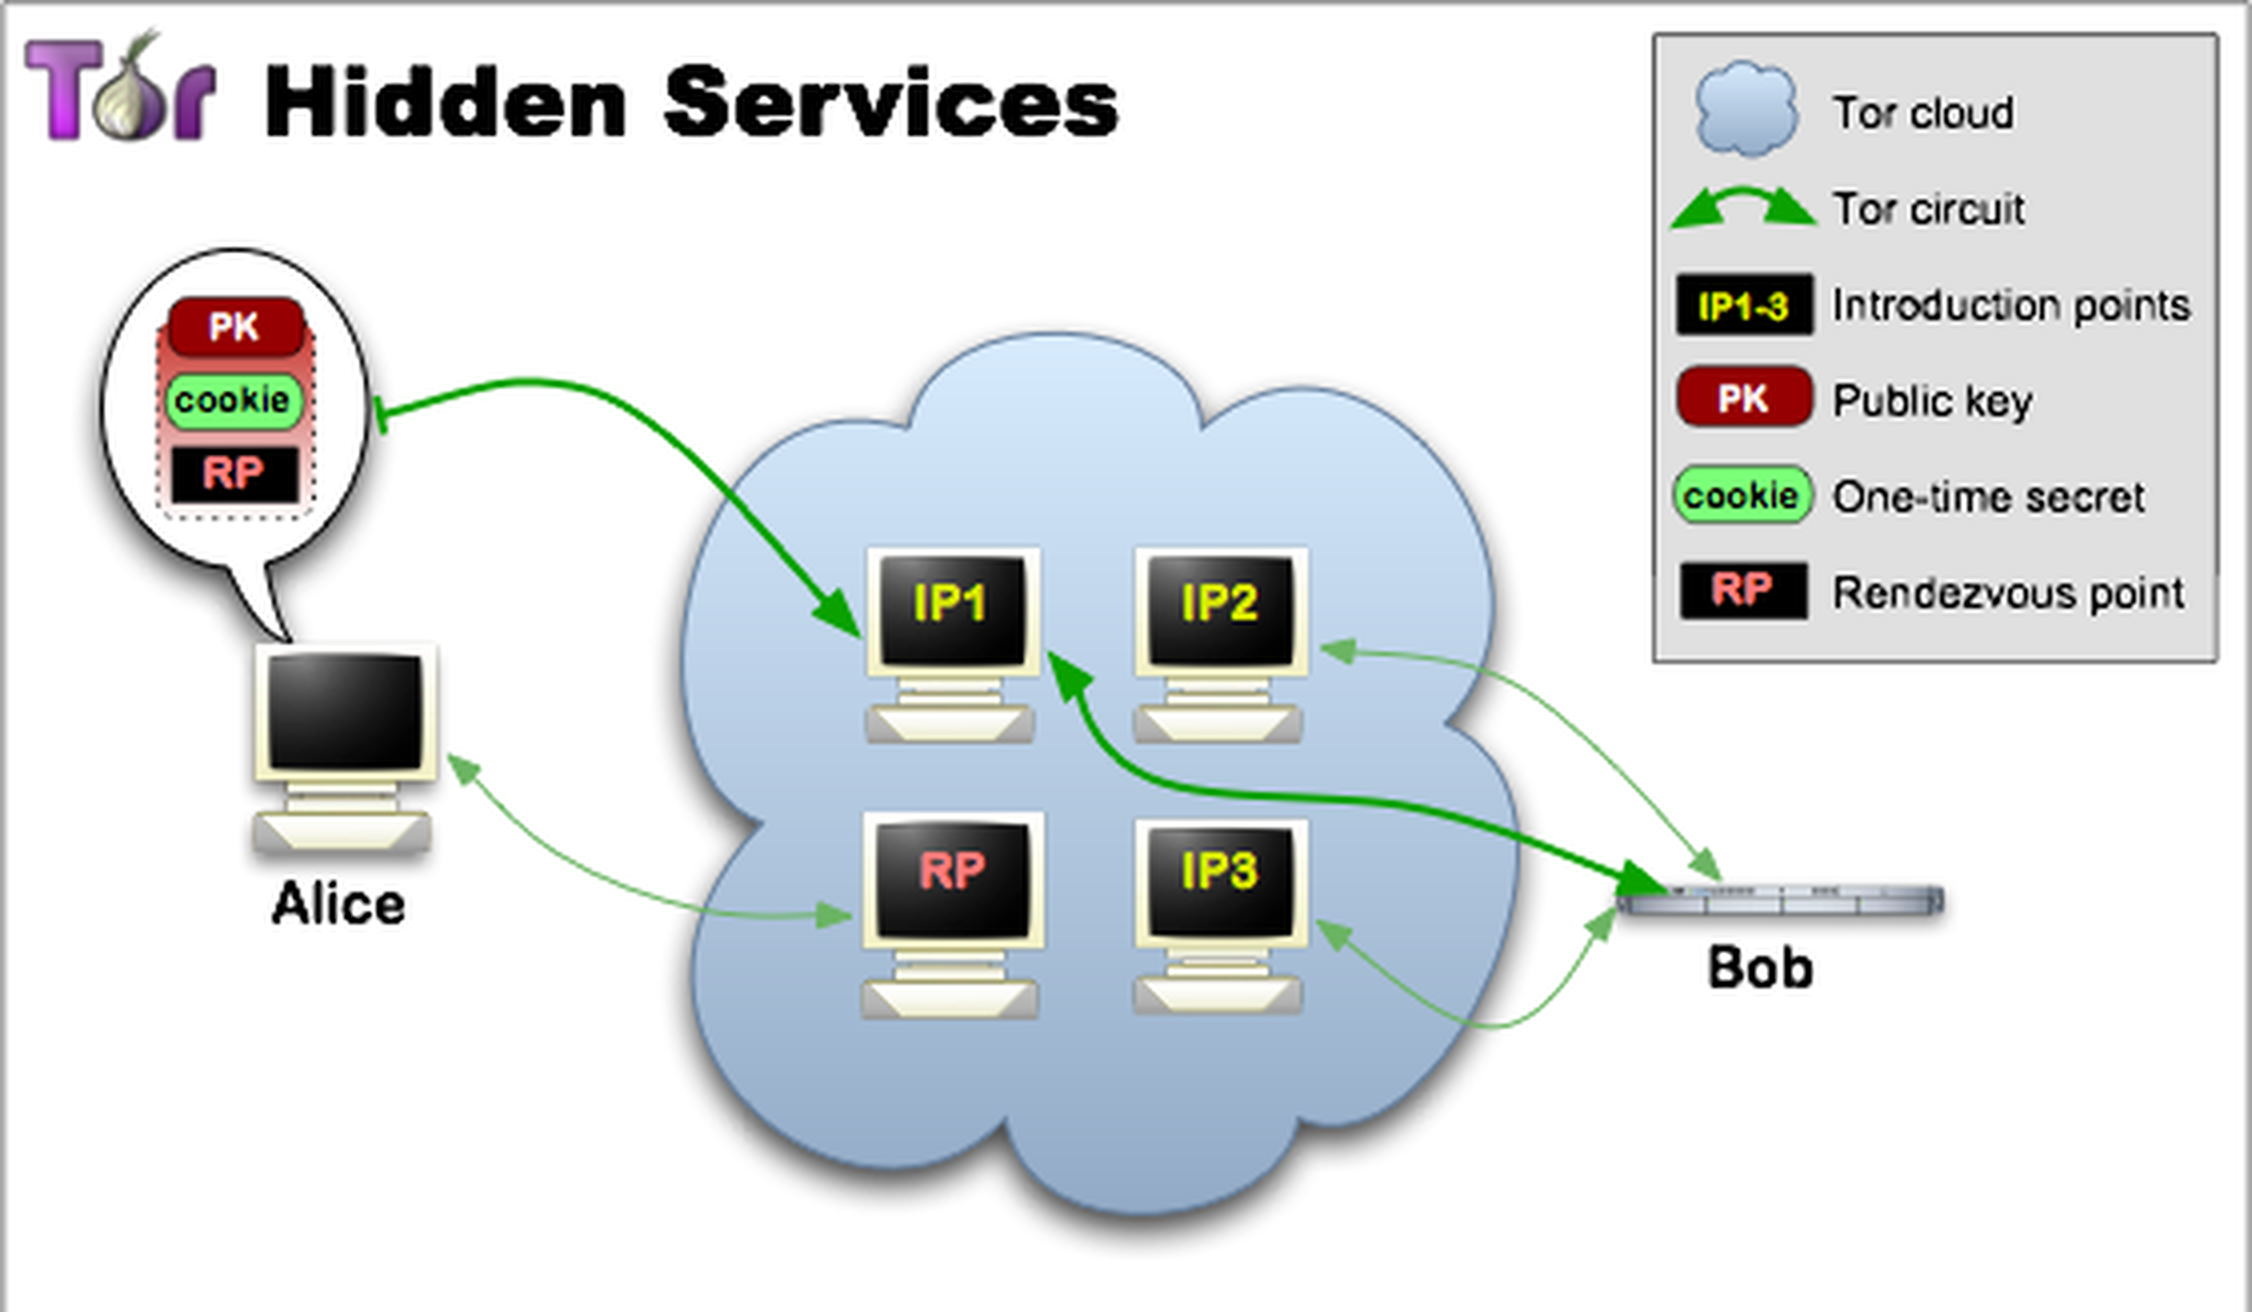
\includegraphics[width=\textwidth]{images/tor-hidden-service-4-higher.png}
		\caption{Alice uses the encrypted cookie to tell Bob to switch to $RP$.}
		\label{fig:figure4}
	\end{minipage}
	\hspace{0.5cm}
	\begin{minipage}[b]{0.45\linewidth}
		\centering
		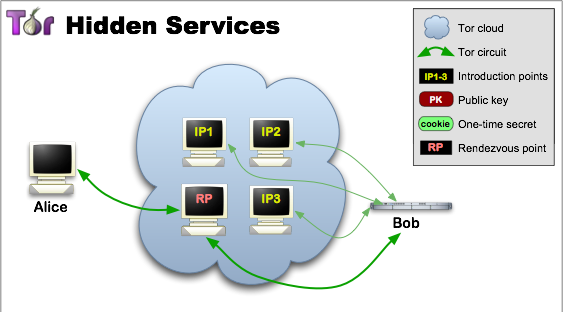
\includegraphics[width=\textwidth]{images/tor-hidden-service-6.png}
		\caption{Bidirectional communication between Alice and the hidden service.}
		\label{fig:figure5}
	\end{minipage}
\end{figure}

She then sends to $IP_{1}$ an cookie encrypted with $B_{K}$, containing $RP$ and $S$. Bob decrypts this message, builds a circuit to $RP$, and tells it $S_{1}$, enabling Alice and Bob to communicate. Their communication travels through six Tor nodes: three established by Alice and three by Bob, so both parties remain anonymous.





% TODO: expand: I spend six pages on Tor + hidden services, I should spend six pages on BTC + Namecoin, and two on DNS
% question: I'm aiming for 50 pages, and it looks I'll be burning 14 or 15 on introductions. Is that all right? If not, reduce to 5 + 5 + 1
\section{Bitcoin} 

Bitcoin is a decentralized peer-to-peer digital cryptocurrency, created by pseudonymous developer Satoshi Nakamoto in 2008. Ownership of Bitcoins consists of holding a private ECDSA key, and a transfer is a transmission of Bitcoins from one key to another. All transactions are recorded on a public ledger, called a blockchain, a data structure whose integrity is ensured through computational power but publically verifiable. Bitcoins are generated computationally at a fixed rate by \textit{miners} in a process that also secures the blockchain. Although Bitcoin received limited attention in the first two years of its life, it has since grown significantly since then, with approximately 70,000 daily transactions as of the time of this writing. Bitcoin's growth has led to the creation of many alternative cryptocurrencies, and its popularity has influenced financial discussions and legal controversy worldwide.

\subsection{Architecture}

A blockchain is data structure fundamental to Bitcoin, and crucial for its functionality. As a distributed decentralized system, this public ledger is Nakamoto's answer to the problem of ensuring agreement of critical data across all involved parties. The blockchain is a novel structure, and its structure guarantees integrity, chronological ordering of transactions, and the prevention of double-spending of Bitcoins. The blockchain consists of blocks of data that are held together by proof-of-work, a cryptographic puzzle whose solution is provably hard to find but trivial to verify. Bitcoin's proof-of-work is based on Adam Back's Hashcash scheme: that is, find a nonce such that the hash of this nonce and some data produces a result that begins with a certain number of zero bits. In Bitcoin's case this is stated as finding a nonce that when passed through two rounds of SHA256 ($ \textrm{SHA}256^{{2}} $) produces a value less than or equal to a target $ T $. This requires a party to perform on average $ \frac{1}{Pr[H \leq T]} = \frac{2 ^ {{256}}}{T} $ amount of computations, but it is easy to verify that $ \textrm{SHA}256^{{2}}(\textrm{msg} || n) \leq T $. Nodes in the Bitcoin network collectively agree to use the blockchain with the highest accumulation of computational effort, so an adversary seeking to modify the structure would need to recompute the proof-of-work for all previous blocks as well as out-perform the network, which is currently considered infeasible.\cite{Okupski2014}

Each block in the blockchain consists of a header and a payload. The header contains a hash of the previous block's header, the root hash of the Merkle tree built from the transactions in this block, a timestamp, a target $ T $, and a nonce. The block payload consists of a list of transactions. The root node of the Merkle tree ensures the integrity of the transaction vector: verifying that a given transaction is contained in the tree takes $ log(n) $ hashes, and a Merkle tree can be built $ n * log(n) $ time, ensuring that all transactions are accounted for. The hash of the previous block in the header ensures that blocks are ordered chronologically, and the Merkle root hash ensures that the transactions contained in each block are order chronologically as well. The target $ T $ changes every 2016 blocks in response to the speed at which the proof-of-work is solved such that Bitcoin miners take two weeks to generate 2016 blocks, or one block every 10 minutes. The $ \textrm{SHA}256^{{2}} $ proof-of-work provides integrity of the data structure, and secp256k1 ECDSA key are used to prove ownership of coins.\cite{Okupski2014}

\begin{figure}[htbp]
	\centering
	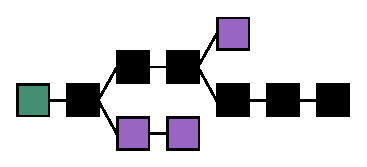
\includegraphics[width=0.6\textwidth]{images/Blockchain-2.eps}
	\caption{A sample blockchain.}
	\label{fig:figure6}
\end{figure}

\begin{figure}[htbp]
	\centering
	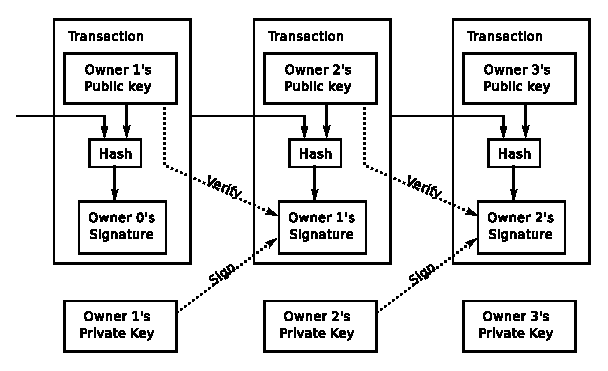
\includegraphics[width=0.6\textwidth]{images/bitcoin_transaction.eps}
	\caption{Three traditional Bitcoin transactions.}
	\label{fig:figure7}
\end{figure}

In the possibility that multiple nodes solve the proof-of-work and generate a new block simultaneously, the block becomes orphaned, the transactions recycled, and the blockchain follows the longest path from the genesis node to the latest block. Each transaction contains the public of the recipient, the ECDSA digital signature of the transaction from the sender, and the hash of the originating transaction. In this way, the digital signatures and proof-of-work in the blockchain can be traced back to the origin and forwards indefinitely. %In practice transactions can contain multiple input and outputs.





\section{Namecoin}

Namecoin is a decentralized information registration and transfer system based on Bitcoin. It was the first software fork of Bitcoin and was introduced in April 2011. It uses its own blockchain and can hold name-value pairs in the blockchain attached to coins. While Bitcoin is primarily focused on supporting a currency, Namecoin aims to be a general key-value store, capable of holding cryptographic keys, DNS registrations, or other arbitrary data. It is most commonly used as a secure and censorship-resistance replacement for clearnet DNS. In 2014, Namecoin was recognized by ICANN is the most well-known example of a PKI and DNS system with an emphasis of distributed control and privacy, a growing trend in light of the revelations about the US Government by Edward Snowden. %https://www.icann.org/en/system/files/files/report-21feb14-en.pdf

\subsection{Names}

Although it inheriting Bitcoin's existing infrastructure, Namecoin added several transaction types specifically for registering and processing names, along with two new rules: names in the blockchain expire after 36,000 blocks unless renewed by the owner and no two unexpired names can be identical. These rules are enforced in the blockchain by Namecoin nodes and anyone verifying the Namecoin blockchain. Registering a name consumes 0.01 Namecoin, names can also be transferred to other owners, and they are two types: DNS and personal. The DNS type uses a new Top Level Domain (TLD) not in use by ICANN: .bit, and is used for DNS registrations. The personal name can contain arbitary data, including user information such as cryptographic keys. Like Bitcoin, Namecoin's maximum block size is one megabyte and the difficulty is set such that blocks generate every 10 minutes. Thus names expire every 250 days. 





\section{DNS}

The Internet Domain Name Service (DNS) is a hierarchical distributed naming system for computers connected to the Internet. It links two principal Internet namespaces, Internet  Protocol (IP) addresses and domain names, and translates one to the other. IP addresses specify the location of a computer or device on a network and domain names identify that resource. Domain names also serve as an abstraction layer so that devices can be moved to a different physical location or to a different IP address without loss of functionality. In contrast to IP addresses, domain names are human-meaningful and easily memorized, so DNS is a crucial component to the usability of the Internet.

Domain names on the Internet consist of a sequence of labels, delimited by dotes. The right-most label is the top-level domain (TLD) and can be used to classify the Internet resource by country or by organization type, although generic TLDs are more common. One or more subdomains follow the TLD. Each label can consist of up to 63 characters and the domain names can be up to 253 characters.  





\section{Zooko's Triangle}

Zooko's Triangle is an influential conjecture proposed by Zooko Wilcox-O'Hearn in late 2001. % Security Usability of Petname Systems http://persons.unik.no/josang/papers/FJSB2009-NordSec.pdf
The conjecture states that in a persistent naming system, only two out of three properties can be established; 

\begin{itemize}
  \item Human meaningfulness: the names have a quality of meaningfulness and memorability to the users of the system. 
  \item Securely one-to-one: each name is unique, corresponds to a unique entity or owner, and cannot be forged or mimicked.
  \item Distributed: the naming system lacks a central authority or database for allocating and distributing names.
\end{itemize}

\begin{figure}[htbp]
	\centering
	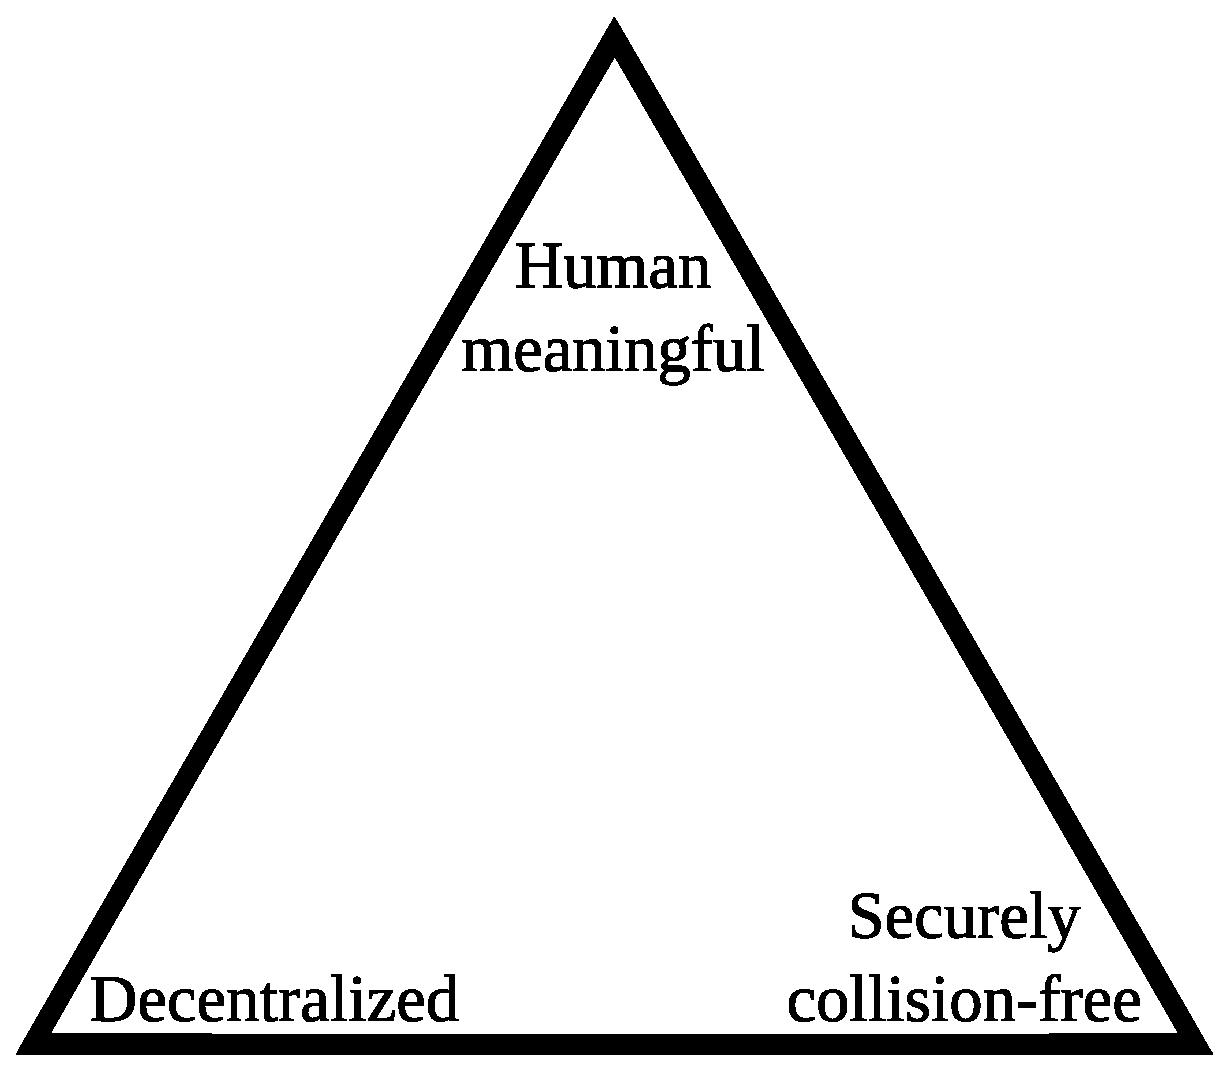
\includegraphics[width=0.4\textwidth]{images/Zooko.eps}
	\caption{Zooko's Triangle.}
	\label{fig:figure8}
\end{figure}

For example, Tor hidden service .onion addresses and Bitcoin addresses are secure and decentralized but are not human-meaningful. Internet domain names are memorable and provably collision-free, but use central database managed DNS under the jurisdiction of ICANN. Finally, human nicknames are meaningful and distributed, but not securely collision-free. %http://www.hpl.hp.com/techreports/2005/HPL-2005-148.pdf Petname Systems

In January of 2011, Aaron Swartz described a naming system based on Bitcoin that achieved all three properties and thus completed Zooko's Triangle. Three months later Namecoin was released as a proof-of-concept, becoming the first system to violate the conjecture. As described above, it allowed human-meaningful key-value pairs (names) to be secured in a global blockchain by proof-of-work, and specified that the uniqueness of the names be verified by a distributed network of miners and confirmation nodes.



%Providing better confidentiality and authentication on the Internet using Namecoin and MinimaLT


\section{Summary}

In this thesis, I utilize the Namecoin blockchain to implement a distributed DNS system that provides human-meaningful and provably unique names to Tor hidden services.

